\documentclass[a4paper,12pt]{article}
\usepackage[utf8]{inputenc}
\usepackage[russian]{babel}
\usepackage{graphicx}
\usepackage{geometry}
\usepackage{hyperref}
\geometry{left=2cm,right=2cm,top=2cm,bottom=2cm}

\begin{document}

\section*{Отчет по домашнему заданию №1}
\subsection*{Курс: «Введение в архитектуру вычислительных систем»}

\subsection*{1. ФИО}
Манро Эйден Форбс (\href{mailto:manro.e@phystech.edu}{manro.e@phystech.edu})

\subsection*{2. Номер группы}
Б01-307

\subsection*{3. Название схемы}
D Flip-Flop (D-триггер)

\subsection*{5. Назначение схемы}
D Flip-Flop — синхронный триггер, сохраняющий состояние входа D на выходе Q при каждом положительном фронте сигнала CLK. Выход !Q является инверсией Q. \\

\textbf{Входы:}
\begin{itemize}
    \item D (данные),
    \item CLK (тактирующий сигнал).
\end{itemize}

\textbf{Выходы:}
\begin{itemize}
    \item Q (сохраненное значение),
    \item !Q (инвертированный Q).
\end{itemize}

\textbf{Принцип работы:}
\begin{itemize}
    \item При переходе CLK из 0 в 1 значение D передается на Q.
    \item В остальное время Q сохраняет предыдущее состояние.
\end{itemize}

\subsection*{6. Скриншоты схемы}

\begin{figure}[h!]
    \centering
    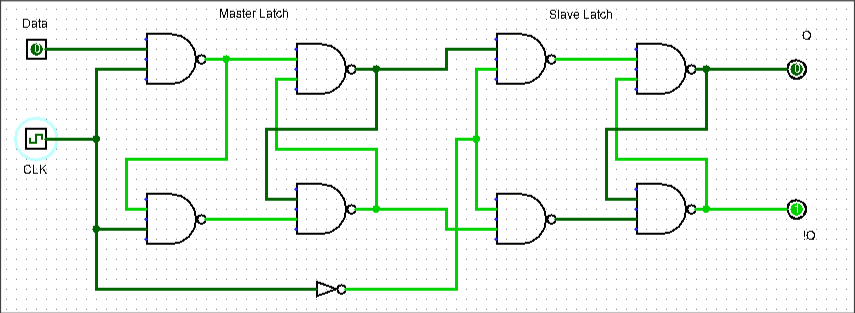
\includegraphics[width=0.8\textwidth]{pictures/dff_0.png}
    \caption{Состояние 1: CLK=0, D=0 → Q сохраняет предыдущее значение.}
\end{figure}

\begin{figure}[h!]
    \centering
    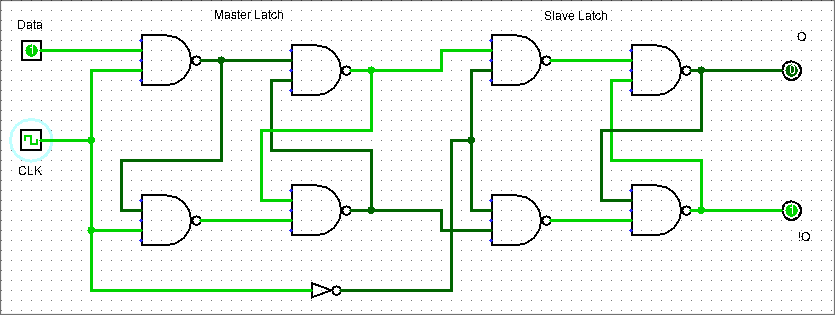
\includegraphics[width=0.8\textwidth]{pictures/dff_1.png}
    \caption{Состояние 2: CLK=1, D=1 → Q=0, CLK сработал раньше, чем D.}
\end{figure}

\begin{figure}[h!]
    \centering
    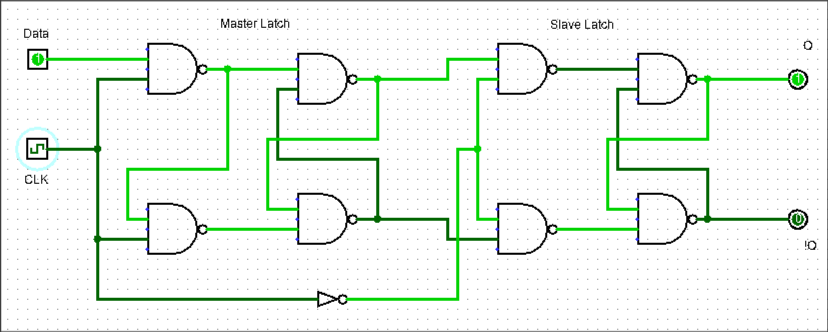
\includegraphics[width=0.8\textwidth]{pictures/dff_2.png}
    \caption{Состояние 3: CLK=0, D=1 → Q=1, CLK сбросился, упс.}
\end{figure}

\begin{figure}[h!]
    \centering
    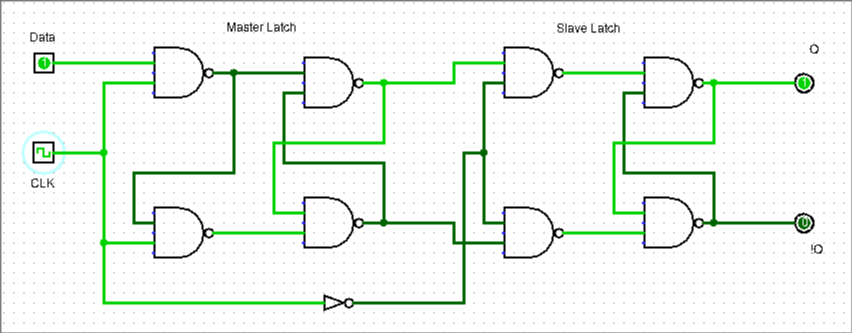
\includegraphics[width=0.8\textwidth]{pictures/dff_3.png}
    \caption{Состояние 4: Все входы в 1 → Q=1.}
\end{figure}

\subsection*{7. Подсчет транзисторов}
Схема D Flip-Flop на основе NAND-элементов и 1 инвертора:
\begin{itemize}
    \item Каждый NAND: 4 транзистора.
    \item Всего NAND-элементов: 8.
    \item Инвертор: 2 транзистора (p и n тип).
\end{itemize}

\textbf{Итого}: \(8 \times 4 \; + \; 2 = 32\) транзистора.

\subsection*{8. Критический путь}
\begin{figure}[h!]
    \centering
    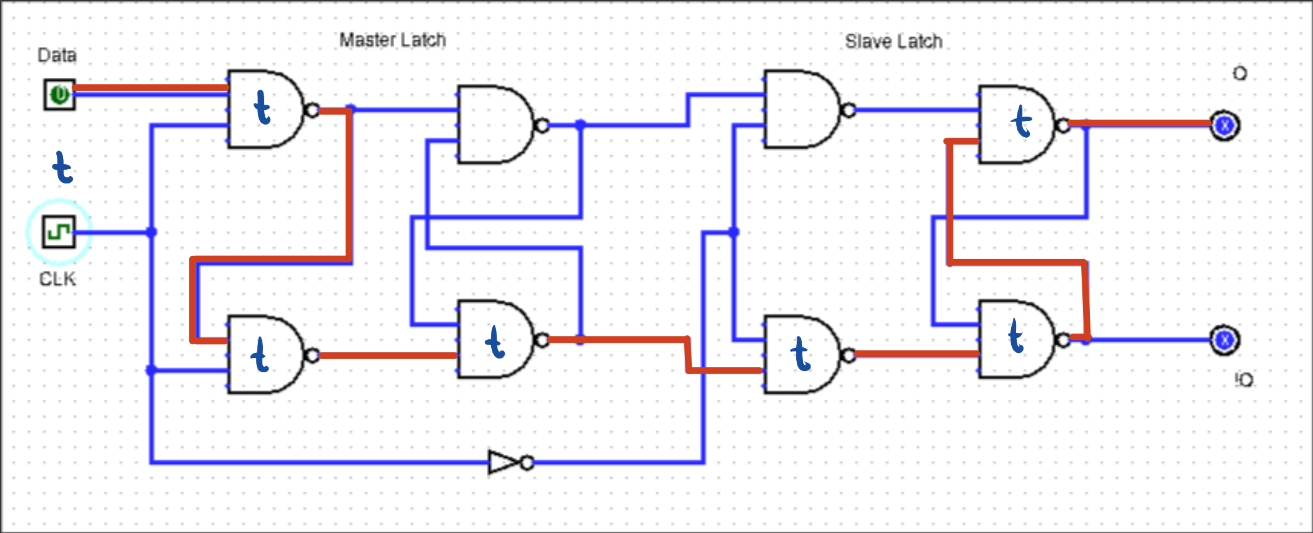
\includegraphics[width=0.8\textwidth]{pictures/crit_path.png}
    \caption{Красной линией выделен путь: D → внутренние элементы → Q. Задержка определяется комбинацией вентилей.}
\end{figure}

$$
    t_{crit\_path} = 3t \; (Master \; Latch) + t \; (CLK) + 3t \; (Slave \; Latch) = 7t
$$

\subsection*{9. Приложенный файл}
Файл схемы: \texttt{flipflop.circ}

\end{document}